\documentclass[conference]{IEEEtran}
\usepackage{newtxtext,newtxmath}
\usepackage{graphicx,booktabs,amsmath,url,cite,xcolor,array,multirow}
\usepackage[hidelinks]{hyperref}

\newcommand{\MemA}{Tathagat Harsh}  \newcommand{\RollA}{2401010477}
\newcommand{\MemB}{M S Thejas}      \newcommand{\RollB}{2401010255}
\newcommand{\MemC}{Garv Verma}      \newcommand{\RollC}{2401010168}
\newcommand{\MemD}{Parv Goyal}      \newcommand{\RollD}{2401010322}
\newcommand{\MemE}{Vaibhav Rajput}  \newcommand{\RollE}{2401010487}
\newcommand{\RepoURL}{https://github.com/TathagatHarsh/dm-cache-controller}
\newcommand{\VideoURL}{https://drive.google.com/drive/folders/1XrK8QC8PR5nWN_Udr-LCHOQUd5ePlpkO?usp=sharing}

\begin{document}
\title{Design, Verification and Evaluation of Direct-Mapped and 2-Way Set-Associative Cache Controllers in Verilog\\
{\large Final Report --- CSA222 Modern Computer Architecture (Project 6)}}
\author{\IEEEauthorblockN{\MemA, \MemB, \MemC, \MemD, \MemE}
\IEEEauthorblockA{\RollA, \RollB, \RollC, \RollD, \RollE\\B.Tech (CS\&AI), Rishihood University / Newton School of Technology}}
\maketitle

\begin{abstract}
We design, verify and evaluate two L1-style cache controllers in synthesizable Verilog: a 1\,KB direct-mapped cache and a 2-way set-associative cache with true LRU replacement. Both use 16-byte blocks, 32-bit addresses, a write-through, no-write-allocate policy, and identical CPU and memory interfaces, so they can be compared on identical traces. A single self-checking testbench with an associativity-generic golden reference model checks the hit/miss outcome, the returned data and the hardware hit/miss counters of every access. Across 22 cache configurations (sizes 256\,B--4\,KB, blocks 8--64\,B, memory latency 5--50 cycles) and eight traces per configuration, 59{,}510 accesses were checked with zero mismatches. At 1\,KB, associativity raises the hit rate of a conflict-heavy trace from 0\% to 98.4\% and the mean workload hit rate from 44.3\% to 64.2\%. The gap closes at 2\,KB and above, where conflicts disappear. Synthesis for a Xilinx Artix-7 target shows the 2-way cache needs about 2$\times$ the LUTs and one extra LUT level on its critical path. Taking clock period into account, the direct-mapped cache still achieves a lower effective access time on the mixed read/write workload. A write-back traffic model shows that write-back halves memory traffic when writes have locality, but nearly doubles it for scattered writes with write-allocate.
\end{abstract}

\begin{IEEEkeywords}
cache memory, direct-mapped cache, set-associative cache, LRU, cache controller, FSM, AMAT, FPGA synthesis, Verilog
\end{IEEEkeywords}

\section{Introduction}
DRAM latency (50--100\,ns) is one to two orders of magnitude longer than a processor clock cycle. This gap is the \emph{memory wall}~\cite{wulf1995}, and computer architects close it with small, fast SRAM caches that exploit temporal and spatial locality~\cite{hp_coa,hp_caqa}. The key design choice is \emph{associativity}. A direct-mapped cache allows each block exactly one location, which makes the hit path as short and cheap as possible but exposes it to conflict misses. A set-associative cache lets a block live in any of $n$ ways, removing most conflict misses at the cost of parallel tag comparators, a way-select multiplexer and replacement state~\cite{hill1988,hill1989}.

\textbf{Objective.} Following Project~6 of the course, we designed and verified a direct-mapped cache controller (Phase~I). In Phase~II we added a 2-way set-associative LRU cache with the same interface and evaluated both on hit ratio, AMAT, memory traffic and FPGA resources across a parameter sweep.

\textbf{Contributions.} (1)~Two synthesizable, modular cache RTL designs that share their storage modules. (2)~A single self-checking testbench whose reference model covers both associativities and every parameter configuration. (3)~A 22-configuration study of capacity, block size and memory latency. (4)~A write-through versus write-back traffic comparison. (5)~Synthesis results and an effective-access-time comparison in the style of Hill~\cite{hill1988}.

\section{Literature Review}
\textbf{Origins.} Wilkes proposed the ``slave memory'' that automatically keeps copies of recently used words~\cite{wilkes1965}. Smith's survey~\cite{smith1982} organized cache design into placement, block size, fetch, replacement and write policy, and used trace-driven simulation to show that small caches capture most references because of locality.

\textbf{Associativity.} Hill~\cite{hill1988} argued that direct-mapped caches can beat set-associative ones in \emph{effective} access time: they have no way-select multiplexer after the tag compare, so the hit path is shorter and the cache can run at a faster clock. Hill and Smith~\cite{hill1989} introduced the 3C model, which divides misses into compulsory, capacity and conflict misses, and showed that associativity mainly removes conflict misses, with diminishing returns as caches grow. Both effects appear directly in our results (Section~\ref{sec:results}).

\textbf{Replacement.} Belady~\cite{belady1966} characterized optimal replacement. LRU is the standard practical approximation, and for two ways it needs only one bit per set. A direct-mapped cache needs no replacement policy, because the victim is fixed by the index.

\textbf{Reducing conflict misses cheaply.} Jouppi~\cite{jouppi1990} kept the direct-mapped hit path and recovered most conflict misses with a small fully-associative victim cache and stream buffers. This middle ground fits naturally between our two designs.

\textbf{Write policies.} Write-through keeps memory consistent and needs no dirty bits, but sends every store to memory, usually through a write buffer. Write-back with write-allocate sends only evicted dirty blocks, at the price of dirty-bit state and more complex eviction~\cite{hp_caqa}. Patterson and Hennessy~\cite{hp_coa} give the four-state controller FSM that our designs adapt.

\textbf{Gap addressed.} Textbooks treat these trade-offs analytically. We build both organizations in IEEE~1364 Verilog~\cite{verilog2005}, verify them cycle by cycle against a reference model, and measure hit ratio, AMAT, traffic and synthesized cost on the same traces.

\section{Proposed Solution}
\subsection{Common Parameters and Interface}
Both caches hold 1\,KB of data in 16-byte (4-word) blocks with 32-bit byte addresses (Table~\ref{tab:params}). All sizes are Verilog parameters. The CPU side is a one-cycle request with \texttt{cpu\_ready}/\texttt{cpu\_hit}. The memory side is a \texttt{mem\_req}/\texttt{mem\_ready} handshake that returns a whole block after $L$ cycles. Hardware counters record hits and misses.

\begin{table}[h]\centering
\caption{Cache organizations (default configuration)}\label{tab:params}
\begin{tabular}{@{}lcc@{}}\toprule
 & Direct-mapped & 2-way LRU \\ \midrule
Lines / sets $\times$ ways & 64 $\times$ 1 & 32 $\times$ 2 \\
Tag / index / offset bits & 22 / 6 / 4 & 23 / 5 / 4 \\
Replacement & none & 1 LRU bit per set \\
Write policy & \multicolumn{2}{c}{write-through, no-write-allocate} \\
Hit time / miss penalty & \multicolumn{2}{c}{1 cycle / $L+1$ cycles} \\ \bottomrule
\end{tabular}\end{table}

\subsection{Direct-Mapped Cache (Phase I)}
The decoder splits the latched address into tag, index and word. The tag, valid and data RAMs are read asynchronously, and the comparator computes $\textit{hit}=\textit{valid}[i]\wedge(\textit{tag}[i]=\textit{tag})$ in a single cycle. The valid bits live in flip-flops so that reset clears every line. A four-state FSM (IDLE, COMPARE, ALLOCATE, WRITE\_MEM) completes read hits in COMPARE, refills on read misses, and forwards every store to memory. On a refill, the requested word is forwarded straight from the memory block.

\subsection{2-Way Set-Associative LRU Cache (Phase II)}
Fig.~\ref{fig:sa2} shows the 2-way design. \textbf{Way storage} instantiates the Phase~I data, tag and valid RAMs once per way, plus a 32-entry LRU bit array that is cleared on reset. \textbf{Way select} compares both tags in parallel ($\textit{hit}_0$, $\textit{hit}_1$), produces \textit{hit}, \textit{hit\_way} and the block of the hitting way, and chooses the \textit{victim}: an invalid way if one exists, otherwise the LRU way. The \textbf{controller} keeps the same four states. In COMPARE it latches the victim, and it updates the set's LRU bit to the way \emph{not} just used, on every hit and every refill. Write hits update only the hitting way. Write misses allocate nothing and leave LRU unchanged.

\begin{figure}[t]\centering
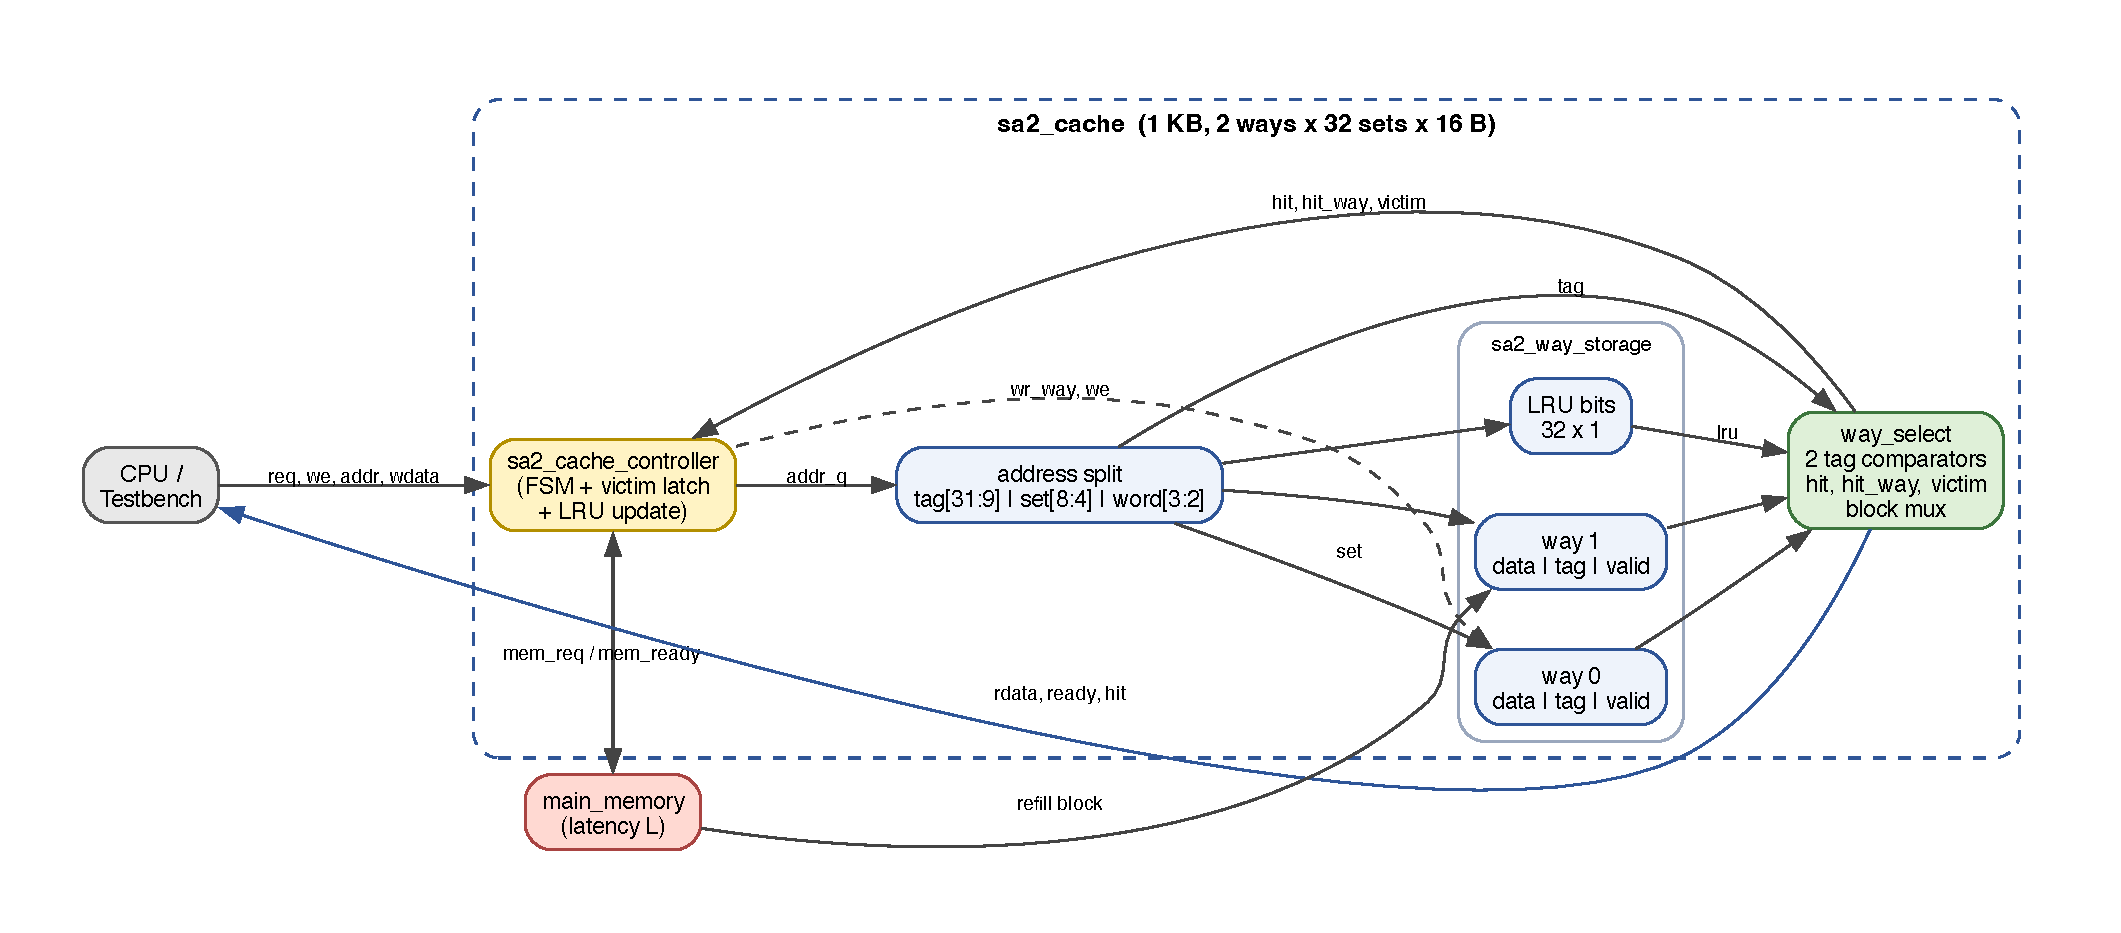
\includegraphics[width=\columnwidth]{../figures/sa2_block_diagram.pdf}
\caption{2-way set-associative LRU cache; the storage modules are reused from the direct-mapped design.}\label{fig:sa2}
\end{figure}

\subsection{Verification Methodology}
\texttt{tb\_cache.v} instantiates either cache, chosen by a parameter, together with a parameterized memory model. Its golden model stores the block address, valid bit and LRU state for each set and way. For every access it predicts hit or miss and the expected data, then compares them with the DUT. At the end of each trace it also compares the totals with the hardware counters. Eight traces are run, each from a cold reset:
\begin{itemize}
\item \textbf{Directed:} cold miss, spatial and temporal hits, write hit, write miss, conflict eviction, and a check that writes reached main memory.
\item \textbf{LRU:} blocks A B A C A B in one set.
\item \textbf{Sequential:} a 2\,KB walk.
\item \textbf{Repeated:} 512\,B read 4 times.
\item \textbf{Random:} 8\,KB, LFSR-generated addresses.
\item \textbf{Conflict:} two blocks 1\,KB apart, alternated.
\item \textbf{Mixed R/W:} 2\,KB, about $3/8$ writes.
\item \textbf{Write loop:} 512\,B written 4 times.
\end{itemize}
A shadow write-back, write-allocate model with the same organization and LRU counts the bytes each policy would move on the memory bus. Every one of the 22 sweep configurations runs all eight traces.

\section{Results and Discussion}\label{sec:results}
\subsection{Functional Verification}
All 22 configurations, 176 trace runs and 59{,}510 checked accesses passed with zero mismatches in hit/miss, data or counters. In the LRU trace the 2-way cache evicts B, not A, when C arrives: miss, miss, hit, miss, hit, miss. This is exactly LRU behavior. The direct-mapped cache misses on all six accesses.

\subsection{Direct-Mapped vs.\ 2-Way at 1 KB}
\begin{table}[t]\centering
\caption{Hit rate and measured read AMAT (1\,KB, 16\,B, $L=10$)}\label{tab:cmp}
\begin{tabular}{@{}lrrrr@{}}\toprule
 & \multicolumn{2}{c}{Hit rate (\%)} & \multicolumn{2}{c}{AMAT (cycles)} \\
Trace & DM & 2-way & DM & 2-way \\ \midrule
Sequential & 75.00 & 75.00 & 3.75 & 3.75 \\
Repeated   & 93.75 & 93.75 & 1.69 & 1.69 \\
Random     & 10.35 & 9.38  & 10.86 & 10.97 \\
Conflict   & 0.00  & \textbf{98.44} & 12.00 & \textbf{1.17} \\
Mixed R/W  & 42.38 & 44.34 & 7.19 & 6.99 \\
LRU (6 acc.) & 0.00 & 33.33 & 12.00 & 8.33 \\ \bottomrule
\end{tabular}\end{table}

Table~\ref{tab:cmp} and Fig.~\ref{fig:pertrace} show the effect of associativity. The sequential and repeated traces are unaffected: one compulsory miss per block and a working set that fits are independent of placement. The conflict trace collapses from 0\% to 98.4\%, because the two blocks share a direct-mapped line but fit in the two ways of a set. This is a pure conflict-miss effect~\cite{hill1989}. Random is slightly \emph{worse} with two ways (9.38\% vs.\ 10.35\%). The 8\,KB working set is capacity-bound, and halving the number of sets changes which blocks collide, so LRU gains nothing here. Measured AMAT equals $1+m(L+1)$ in every case, which confirms the cycle timing of both controllers.

\begin{figure}[t]\centering
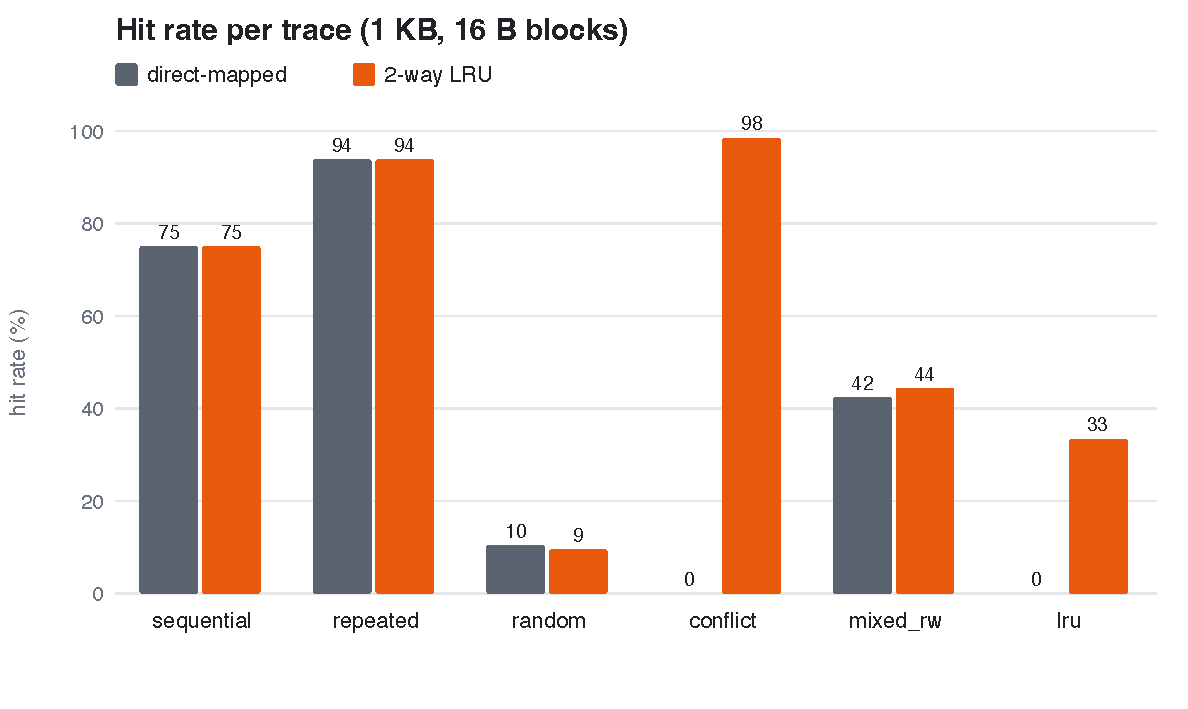
\includegraphics[width=\columnwidth]{../figures/p2_hit_per_trace.pdf}
\caption{Per-trace hit rate of both caches at 1\,KB.}\label{fig:pertrace}
\end{figure}

\subsection{Capacity, Block Size and Latency}
Fig.~\ref{fig:size} shows the mean hit rate of the five workload traces. The 2-way cache leads by about 19--20 points up to 1\,KB (52.8\% vs.\ 33.6\% at 256\,B; 64.2\% vs.\ 44.3\% at 1\,KB). The two curves meet at 2\,KB, where the conflict trace's blocks fall into different direct-mapped lines. Associativity pays most when the cache is small relative to the conflicting footprint, as Hill and Smith observed~\cite{hill1989}.

\begin{figure}[t]\centering
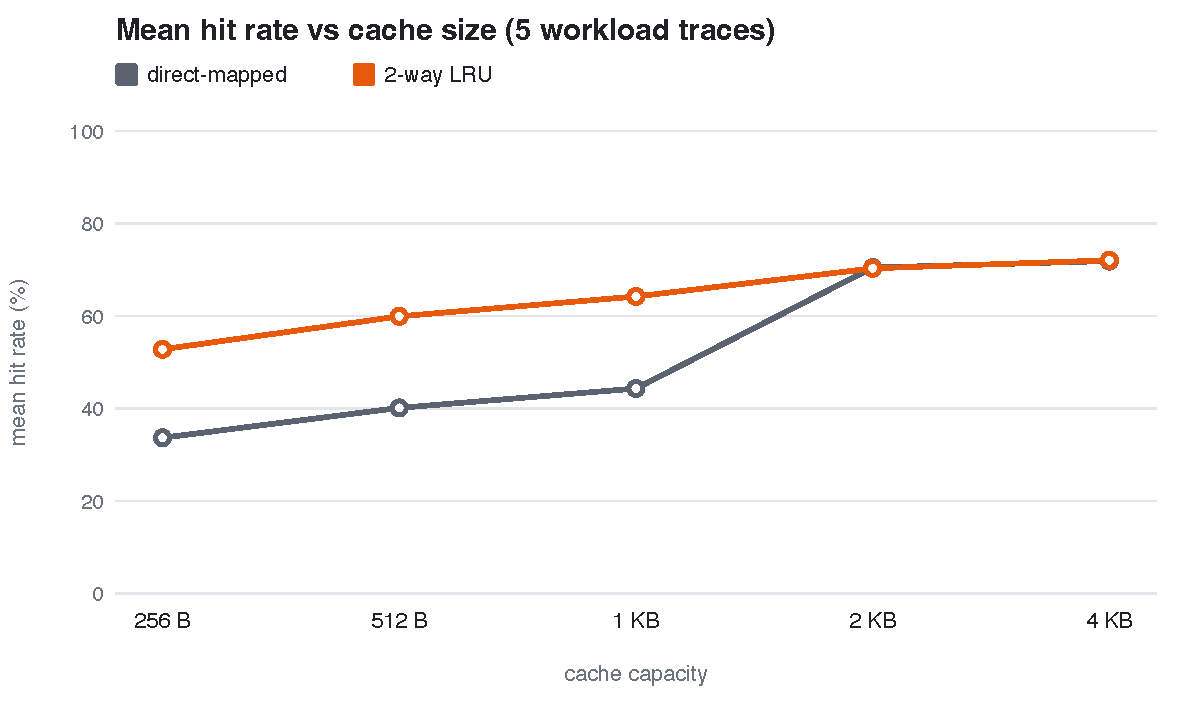
\includegraphics[width=\columnwidth]{../figures/p2_hit_vs_size.pdf}
\caption{Mean hit rate vs.\ capacity (16\,B blocks, $L=10$).}\label{fig:size}
\end{figure}

Larger blocks raise the sequential hit rate from 50\% (8\,B) to 93.75\% (64\,B), since one miss brings in more neighbors (Fig.~\ref{fig:block}). On the mixed workload the hit rate peaks at 32\,B (48.4\%) and falls at 64\,B. With only 16 lines left, conflicts and wasted fetched words outweigh the spatial benefit. Our memory model returns any block size in the same $L$ cycles. Real DRAM spends longer transferring larger blocks, which would move the optimum toward smaller blocks.

\begin{figure}[t]\centering
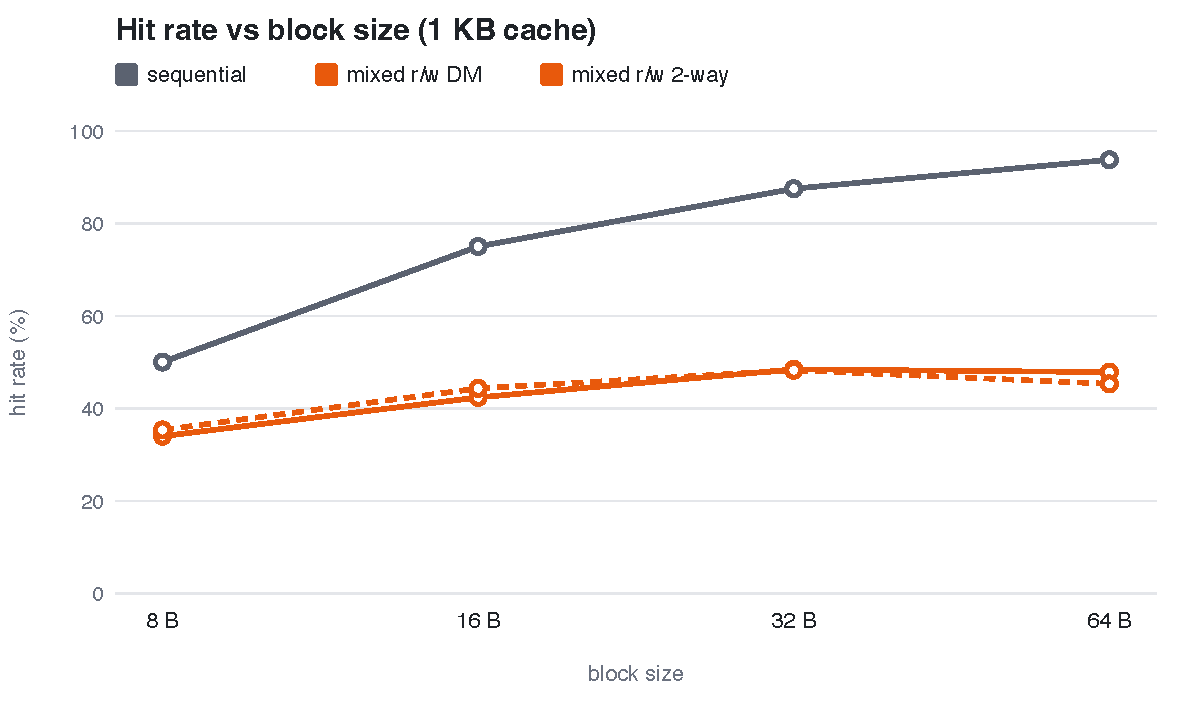
\includegraphics[width=\columnwidth]{../figures/p2_hit_vs_block.pdf}
\caption{Hit rate vs.\ block size (1\,KB).}\label{fig:block}
\end{figure}

AMAT grows linearly with memory latency, and its slope is the miss rate (Fig.~\ref{fig:lat}). On the mixed workload it rises from 4.38 to 29.7 cycles (DM) and from 4.27 to 28.8 cycles (2-way) as $L$ goes from 5 to 50. The 2-way cache's small hit-rate edge becomes a growing absolute advantage as memory gets slower.

\begin{figure}[t]\centering
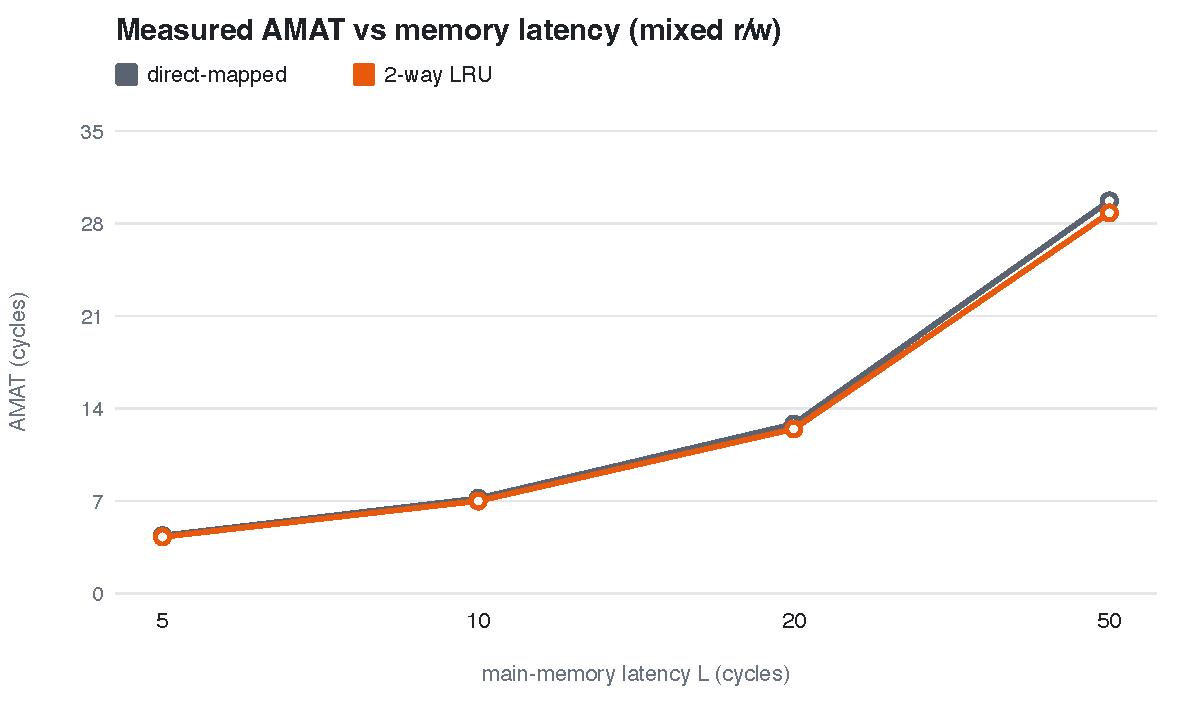
\includegraphics[width=\columnwidth]{../figures/p2_amat_vs_latency.pdf}
\caption{Measured AMAT vs.\ memory latency (mixed R/W, 1\,KB).}\label{fig:lat}
\end{figure}

\subsection{Write-Through vs.\ Write-Back Traffic}
On read-only traces both policies move the same bytes (Fig.~\ref{fig:traffic}). In the write loop, write-back halves the traffic (1{,}024 vs.\ 2{,}048\,B): 32 block fetches and 32 dirty write-backs replace 512 individual word writes. On the mixed workload, write-back with write-allocate moves \emph{more} data (6{,}464 vs.\ 3{,}720\,B), because each scattered write miss fetches a 16-byte block that is never reused. Write-back pays off when stores have locality. Otherwise, write-through with a write buffer, or write-back with no-write-allocate, is the better choice.

\begin{figure}[t]\centering
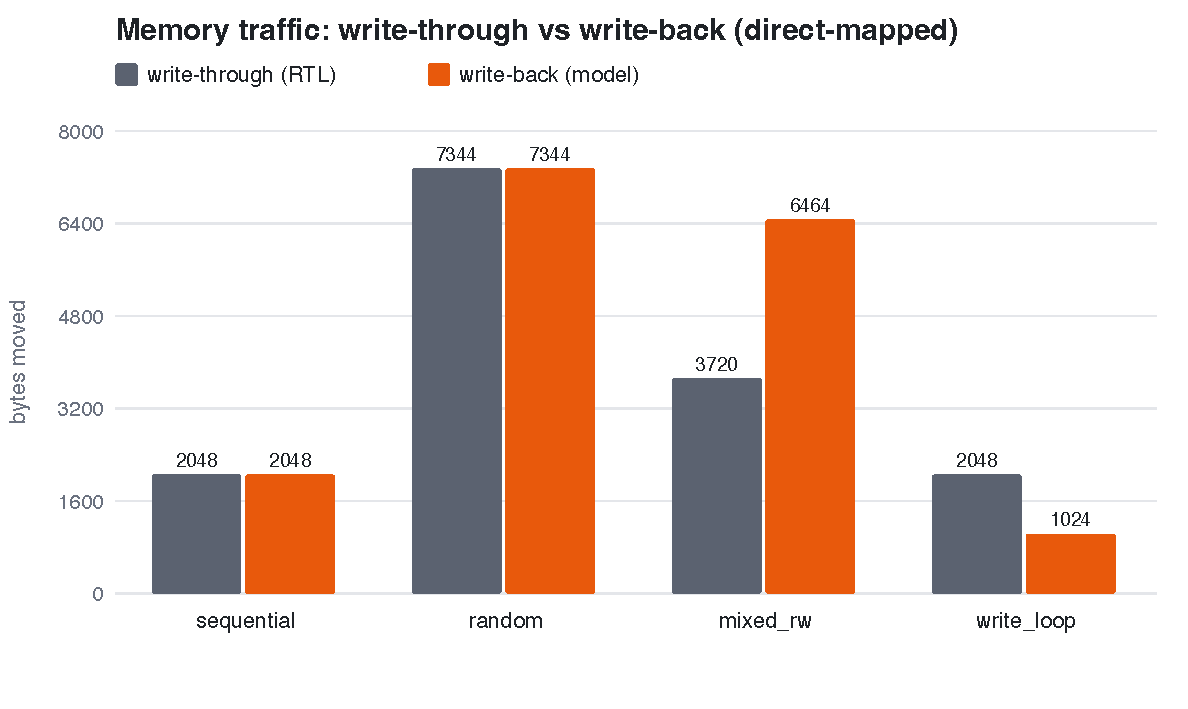
\includegraphics[width=\columnwidth]{../figures/p2_traffic.pdf}
\caption{Bytes on the memory bus: write-through RTL vs.\ write-back model (direct-mapped, 1\,KB).}\label{fig:traffic}
\end{figure}

\subsection{Synthesis and Effective Access Time}
Both tops were synthesized with Yosys~\cite{yosys} (\texttt{synth\_xilinx}, 7-series) for an Artix-7 target (Table~\ref{tab:syn}, Fig.~\ref{fig:res}). Data and tag arrays map to distributed LUTRAM~\cite{ug474}, and valid and LRU bits map to flip-flops. The 2-way cache doubles both the logic LUTs (412 $\rightarrow$ 805) and the LUTRAM (544 $\rightarrow$ 1{,}056 LUTs). Together these are 4.6\% and 8.9\% of the 20{,}800 LUTs of an xc7a35t. The way multiplexer adds one LUT level to the critical path (6 $\rightarrow$ 7 levels, from ABC's mapping).

\begin{table}[t]\centering
\caption{Artix-7 synthesis (Yosys)}\label{tab:syn}
\begin{tabular}{@{}lrr@{}}\toprule
 & DM & 2-way \\ \midrule
Logic LUTs & 412 & 805 \\
LUTRAM (LUTs) & 544 & 1{,}056 \\
Flip-flops & 202 & 234 \\
CARRY4 & 18 & 18 \\
LUT levels on critical path & 6 & 7 \\
Est.\ clock period / $F_{max}$ & 4.9\,ns / $\approx$204\,MHz & 5.4\,ns / $\approx$185\,MHz \\ \bottomrule
\end{tabular}\end{table}

\begin{figure}[t]\centering
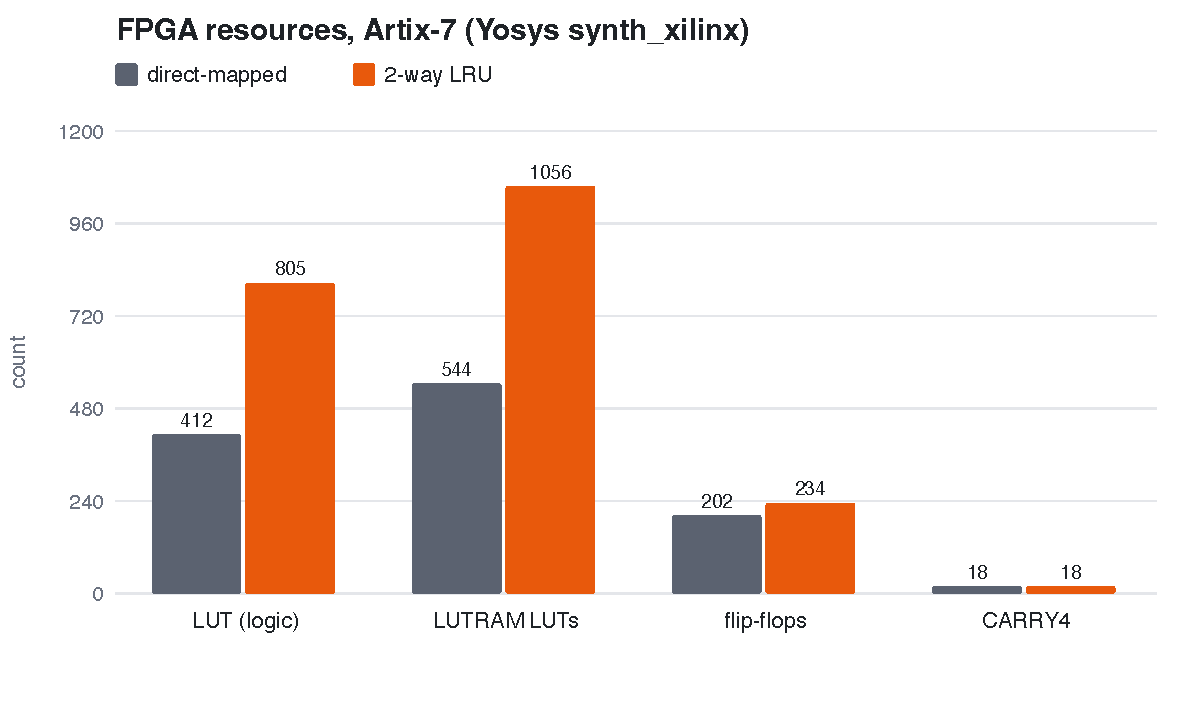
\includegraphics[width=\columnwidth]{../figures/p2_resources.pdf}
\caption{FPGA resources of both caches.}\label{fig:res}
\end{figure}

The $F_{max}$ values are a first-order estimate, not a timing sign-off. They assume about 0.6\,ns of register overhead, about 1.3\,ns for the LUTRAM read and about 0.5\,ns per LUT level including routing. A Vivado script (\texttt{synth/vivado\_synth.tcl}) is provided to obtain exact post-route timing on lab machines.

Following Hill~\cite{hill1988}, we compare \emph{time} rather than cycles. On the mixed workload, the direct-mapped cache needs $7.19\times4.9\approx35.2$\,ns per read against $6.99\times5.4\approx37.7$\,ns for the 2-way cache, so its faster clock outweighs its 2-point hit-rate deficit. On the conflict trace the 2-way cache wins decisively ($1.17\times5.4\approx6.3$\,ns vs.\ $58.8$\,ns). Which design is better therefore depends on the workload's conflict behavior. This is the classic result, here reproduced from measured RTL.

\subsection{Limitations}
$F_{max}$ is estimated, not measured. The write-back figures come from a verified trace model, not RTL. The memory model has fixed latency independent of block size. The traces are synthetic, not from real programs.

\section{Individual Contributions}
\begin{table}[h]\centering
\caption{Work distribution (each member committed their own files)}\label{tab:contrib}
\begin{tabular}{@{}>{\raggedright\arraybackslash}p{0.2\columnwidth}>{\raggedright\arraybackslash}p{0.34\columnwidth}>{\raggedright\arraybackslash}p{0.36\columnwidth}@{}}\toprule
Member & Phase I & Phase II \\ \midrule
\MemA & Controller FSM (\texttt{cache\_controller}), state diagram, README & 2-way controller with victim latch and LRU update (\texttt{sa2\_cache\_controller}); final report \\
\MemB & Data/tag/valid RAMs (\texttt{cache\_rams}); Phase I report & 2-way storage with LRU bits (\texttt{sa2\_way\_storage}); viva preparation notes \\
\MemC & Address decoder, tag comparator, block diagram & Parallel compare, victim select, way mux (\texttt{way\_select}); 2-way block diagram \\
\MemD & Main-memory model, \texttt{dm\_cache} integration, waveforms, film & \texttt{sa2\_cache} top, parameterized memory, Yosys and Vivado synthesis \\
\MemE & Self-checking testbench, traces, results & Generic testbench and reference model, write-back model, sweeps, figures \\ \bottomrule
\end{tabular}\end{table}
Repository: \url{\RepoURL}. Demo video: \url{\VideoURL}.

\section{Conclusion}
We built and exhaustively verified two cache controllers that share storage modules and an interface, and evaluated them over 22 configurations. Associativity is a targeted fix for conflict misses. It turns a 0\% conflict trace into 98\% hits and lifts the mean workload hit rate by about 20 points in small caches, but it adds nothing for streaming or capacity-bound accesses and vanishes once the cache outgrows the conflicting footprint. It costs about 2$\times$ the LUTs and one extra logic level, so the faster direct-mapped cache can still win on effective access time, which supports Hill's argument for direct-mapped caches. Block size trades spatial locality against line count, and write-back only reduces traffic when stores have locality. Natural next steps are post-route timing in Vivado, a victim cache~\cite{jouppi1990}, a write buffer or RTL write-back controller, and replaying instruction and data traces captured from a RISC-V core.

\begin{thebibliography}{99}
\bibitem{wilkes1965} M.~V. Wilkes, ``Slave memories and dynamic storage allocation,'' \emph{IEEE Trans. Electron. Comput.}, vol.~EC-14, no.~2, pp.~270--271, Apr. 1965.
\bibitem{smith1982} A.~J. Smith, ``Cache memories,'' \emph{ACM Comput. Surv.}, vol.~14, no.~3, pp.~473--530, Sep. 1982.
\bibitem{hill1988} M.~D. Hill, ``A case for direct-mapped caches,'' \emph{Computer}, vol.~21, no.~12, pp.~25--40, Dec. 1988.
\bibitem{hill1989} M.~D. Hill and A.~J. Smith, ``Evaluating associativity in CPU caches,'' \emph{IEEE Trans. Comput.}, vol.~38, no.~12, pp.~1612--1630, Dec. 1989.
\bibitem{jouppi1990} N.~P. Jouppi, ``Improving direct-mapped cache performance by the addition of a small fully-associative cache and prefetch buffers,'' in \emph{Proc. 17th Annu. Int. Symp. Comput. Archit. (ISCA)}, 1990, pp.~364--373.
\bibitem{belady1966} L.~A. Belady, ``A study of replacement algorithms for a virtual-storage computer,'' \emph{IBM Syst. J.}, vol.~5, no.~2, pp.~78--101, 1966.
\bibitem{wulf1995} W.~A. Wulf and S.~A. McKee, ``Hitting the memory wall: Implications of the obvious,'' \emph{ACM SIGARCH Comput. Archit. News}, vol.~23, no.~1, pp.~20--24, Mar. 1995.
\bibitem{hp_coa} D.~A. Patterson and J.~L. Hennessy, \emph{Computer Organization and Design: The Hardware/Software Interface}, 5th~ed. Waltham, MA, USA: Morgan Kaufmann, 2014, ch.~5.
\bibitem{hp_caqa} J.~L. Hennessy and D.~A. Patterson, \emph{Computer Architecture: A Quantitative Approach}, 6th~ed. Cambridge, MA, USA: Morgan Kaufmann, 2017, ch.~2 and App.~B.
\bibitem{verilog2005} \emph{IEEE Standard for Verilog Hardware Description Language}, IEEE Std 1364-2005, 2006.
\bibitem{yosys} C.~Wolf, ``Yosys Open SYnthesis Suite,'' [Online]. Available: \url{https://yosyshq.net/yosys/}
\bibitem{ug474} Xilinx, \emph{7 Series FPGAs Configurable Logic Block User Guide}, UG474, 2016.
\end{thebibliography}
\end{document}
